
\documentclass{beamer}  % 添加 dvipdfmx 选项
\usepackage{luatexja} 
\usepackage{hyperref}
\usepackage[T1]{fontenc}

% other packages
\usepackage{latexsym,amsmath,xcolor,multicol,booktabs,calligra}
\usepackage{graphicx,pstricks,listings,stackengine}

% dummy text; remove it when working on this template
\usepackage{lipsum}

\author{Ran YI}
\title{仮想通貨に関しての時系列解析}
\subtitle{}
\institute{
    Department of Mathematical Sciences \\
    Ritsumeikan University
}
\date{\today}
\usepackage{Ritsumeikan}

% defs
\def\cmd#1{\texttt{\color{red}\footnotesize $\backslash$#1}}
\def\env#1{\texttt{\color{blue}\footnotesize #1}}
\definecolor{deepblue}{rgb}{0,0,0.5}
\definecolor{deepred}{rgb}{0.6,0,0}
\definecolor{deepgreen}{rgb}{0,0.5,0}
\definecolor{halfgray}{gray}{0.55}

\lstset{
    basicstyle=\ttfamily\small,
    keywordstyle=\bfseries\color{deepblue},
    emphstyle=\ttfamily\color{deepred},    % Custom highlighting style
    stringstyle=\color{deepgreen},
    numbers=left,
    numberstyle=\small\color{halfgray},
    rulesepcolor=\color{red!20!green!20!blue!20},
    frame=shadowbox,
}


\begin{document}

\begin{frame}
    \titlepage
    \begin{figure}[ht]
        \begin{center}
            
\includegraphics[keepaspectratio, scale=0.017]{pic/Ritsumeikan_University_Logo.png}
        \end{center}
    \end{figure}
\end{frame}

\begin{frame}
    \tableofcontents[sectionstyle=show,subsectionstyle=show/shaded/hide,subsubsectionstyle=show/shaded/hide]
\end{frame}

\section{Introduction}
\begin{frame}{データの準備}
    2018年1月1日から2025年1月1日までのBTC-USDデータを使っている
    \begin{figure}[h]
        \begin{center}
            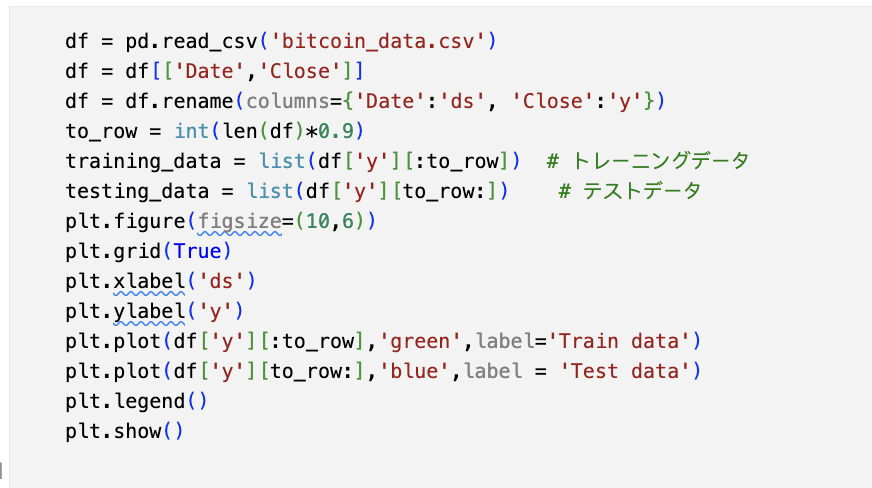
\includegraphics[keepaspectratio, scale=0.5]{pic/data_pre.png}
        \end{center}
    \end{figure}    
\end{frame}


\section{Prophet Model}
\subsection{Facebookが開発した時系列解析用のライブラリー}

\begin{frame}{Facebook Prophetモデルの設定}
    \begin{figure}[h]
        Facebook Prophetの時系列解析モデル\\
        (詳細: https://facebook.github.io/prophet/)
        \begin{center}
            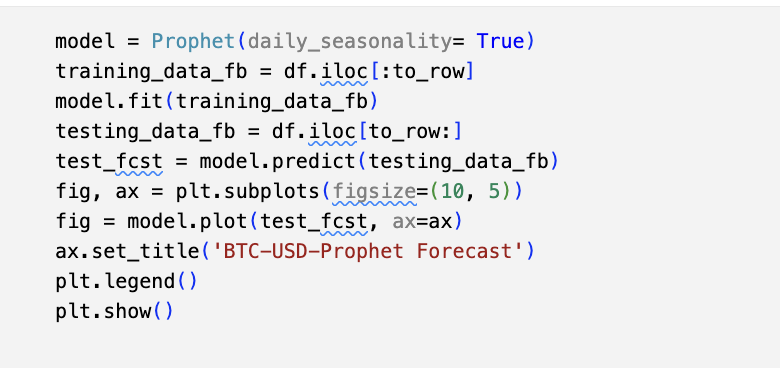
\includegraphics[keepaspectratio, scale=0.6]{pic/pp_set.png}
        \end{center}
    \end{figure}  
\end{frame}

\begin{frame}{一般化予測}
    \begin{figure}[h]
        \begin{center}
            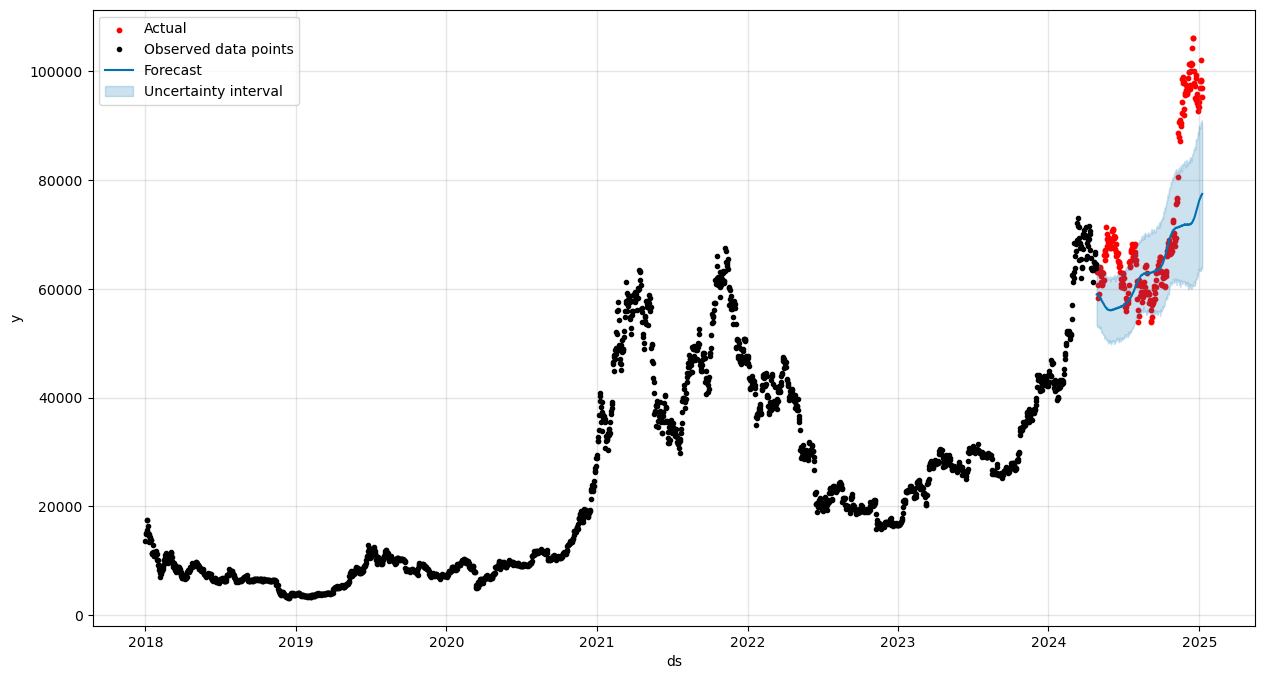
\includegraphics[keepaspectratio, width=0.5\textwidth]{pic/pp_fcst1_1.png}\\
            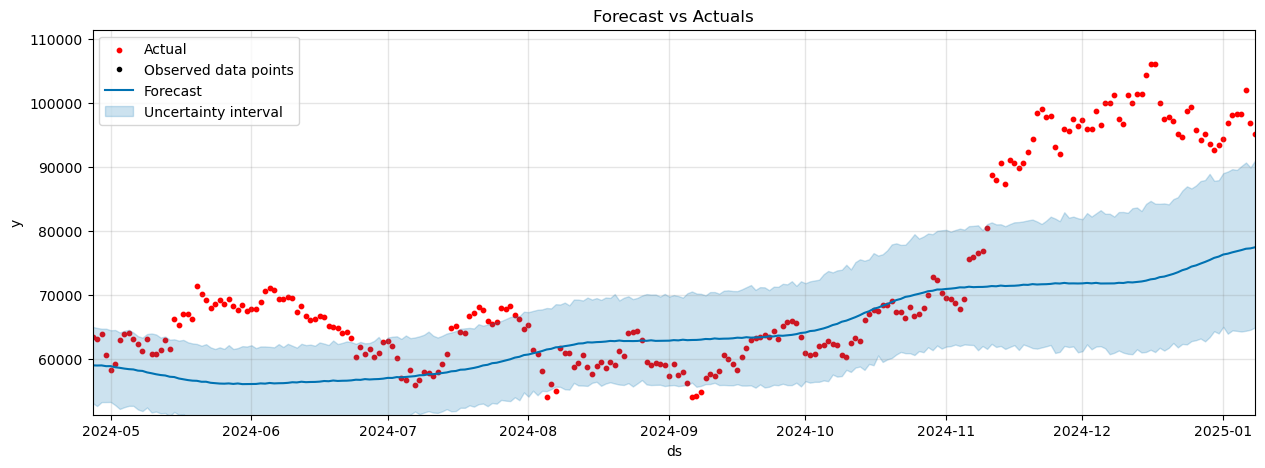
\includegraphics[keepaspectratio, width=0.6\textwidth]{pic/pp_fcst1_2.png}\\
            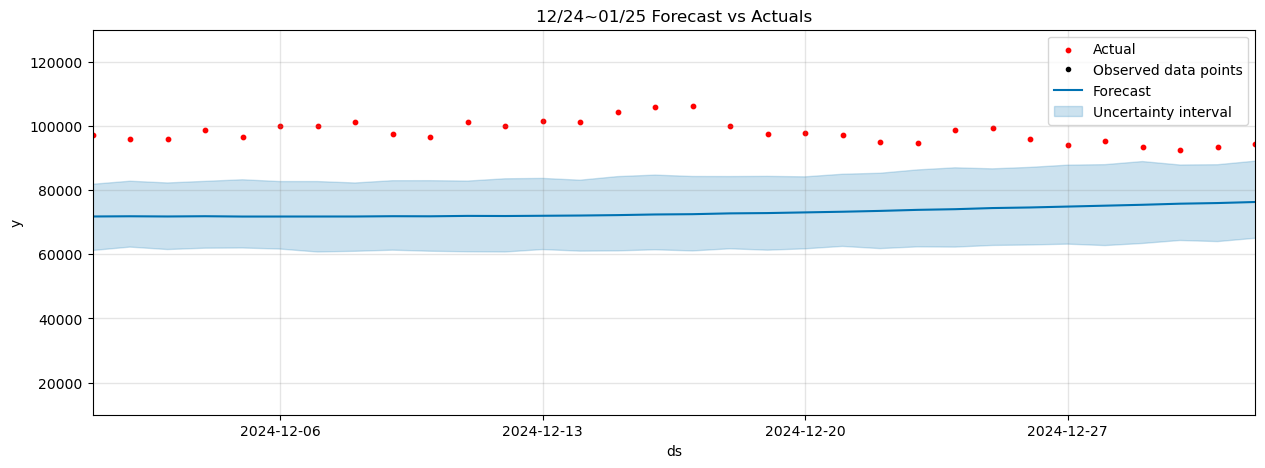
\includegraphics[keepaspectratio, width=0.6\textwidth]{pic/pp_fcst1_3.png}
        \end{center}
    \end{figure}
\end{frame}

\begin{frame}
    \frametitle{年月日のトレンド}
    \begin{figure}[h]
        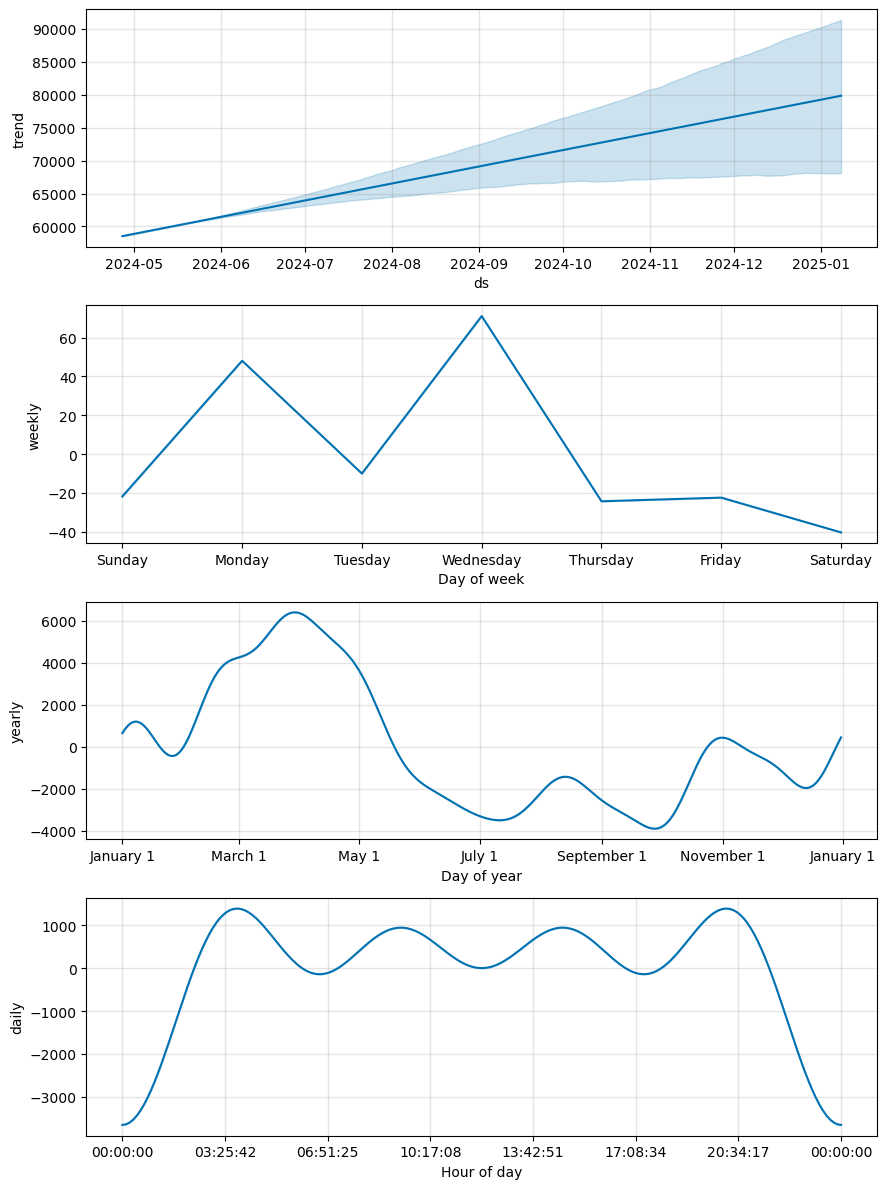
\includegraphics[keepaspectratio, width=0.5\textwidth]{pic/pp_fcst1.png}
    \end{figure}
\end{frame}

\begin{frame}
    \frametitle{モデルの評価}
\begin{itemize}
   \item  MSE Value(平均二乗誤差): 12724.452579794137\\
   \item  MAE Value(平均絶対誤差): 9289.974856441853\\
   \item  MAPE Value(平均絶対パーセント誤差): 11.582111797512047
\end{itemize}
\end{frame}

\begin{frame}
    \frametitle{祝日含みでのモデル訓練}
    \begin{figure}[h]
        \begin{center}
            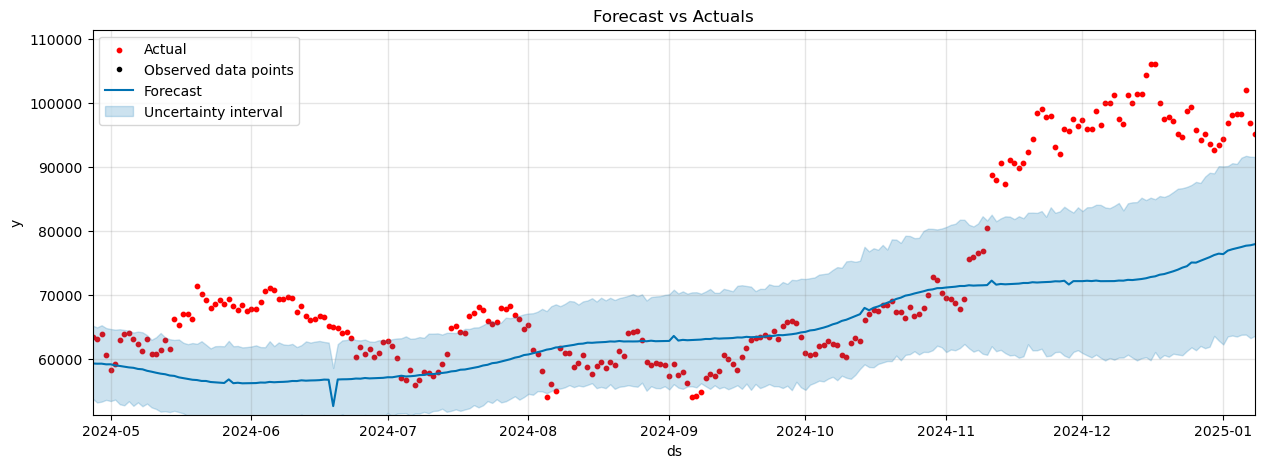
\includegraphics[keepaspectratio, width=0.65\textwidth]{pic/pp_fcst2_1.png}\\
            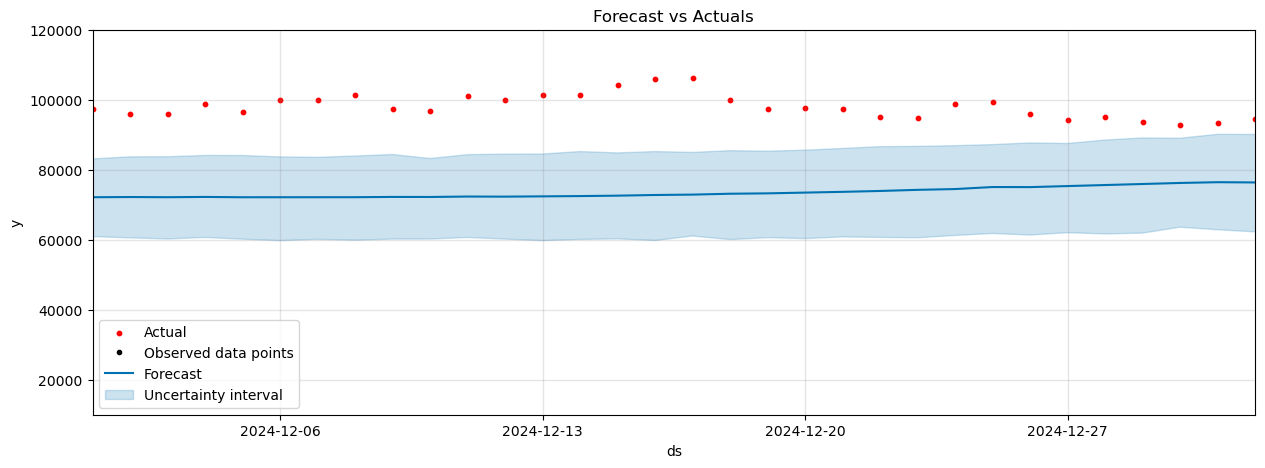
\includegraphics[keepaspectratio, width=0.65\textwidth]{pic/pp_fcst2_2.png}\\
        \end{center}
    \end{figure}
\end{frame}

\begin{frame}
    \frametitle{祝日含み版}
    \begin{figure}[htbp]
        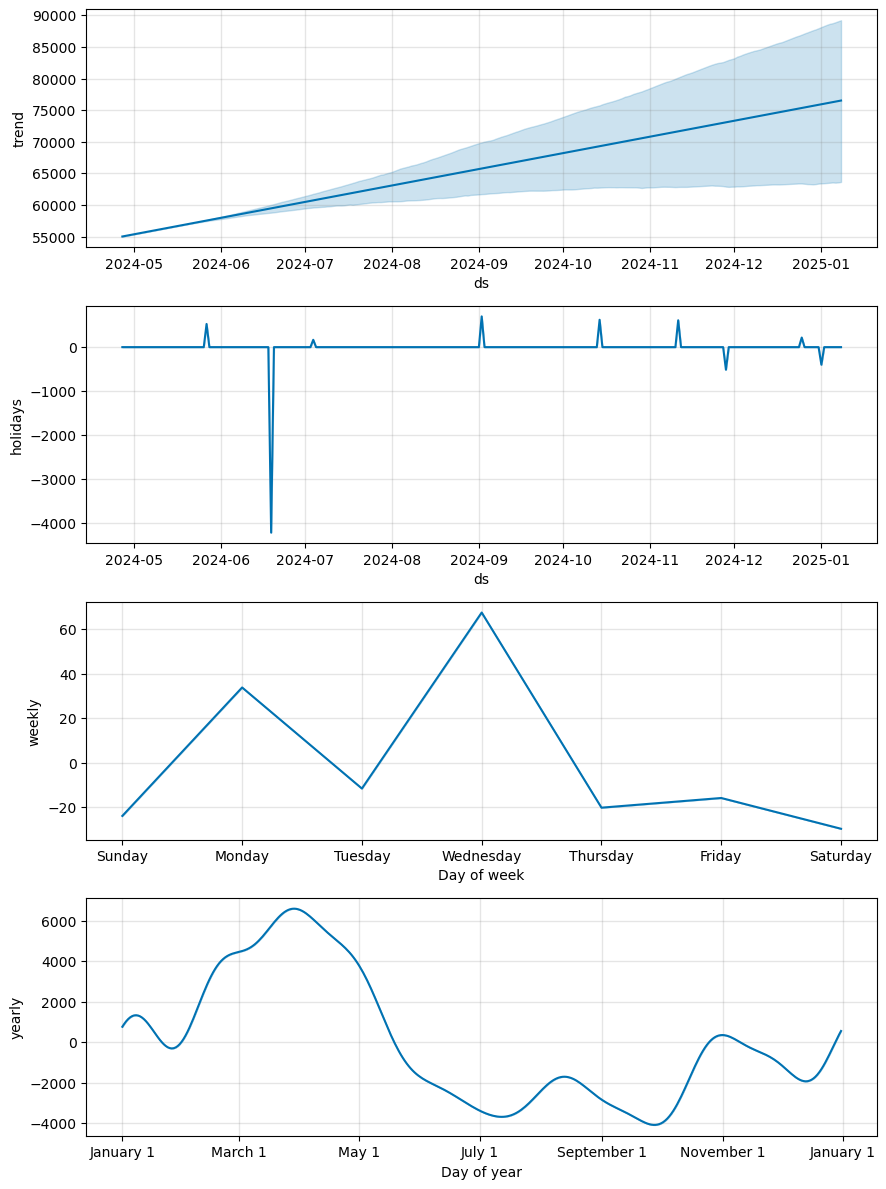
\includegraphics[keepaspectratio, width=0.6\textwidth]{pic/pp_fcst2.png}
    \end{figure}
\end{frame}

\begin{frame}
    \frametitle{祝日版Prophetモデル評価}
    \begin{itemize}
        \item SE Value(平均二乗誤差): 12550.97617585529
        \item MAE Value(平均絶対誤差): 9187.666839253901
        \item MAPE Value(平均絶対パーセント誤差): 11.468800365741414
    \end{itemize}
\end{frame}

\begin{frame}
    \frametitle{未来1年の予測}
    \begin{figure}[h]
        \begin{center}
            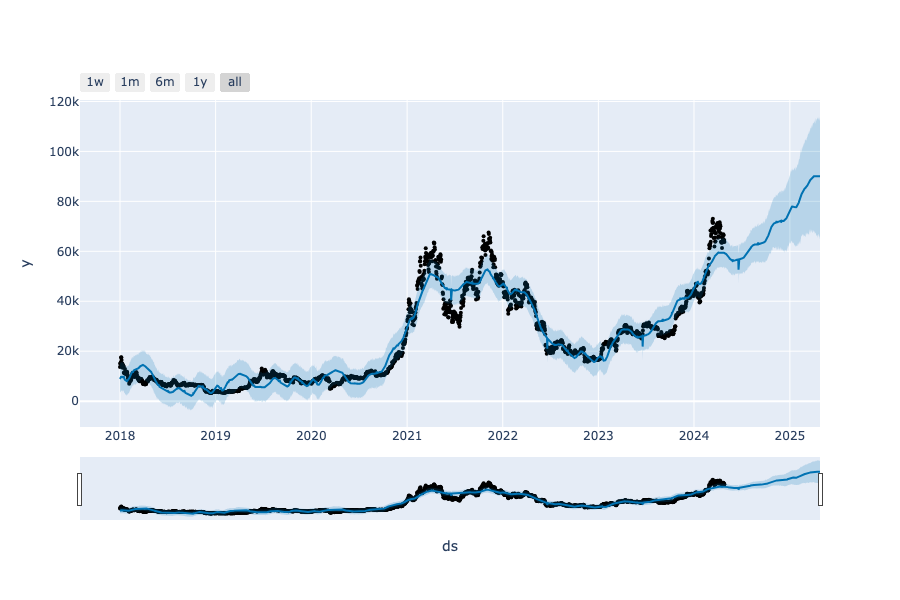
\includegraphics[keepaspectratio, width=0.95\textwidth]{pic/prophet_all.png}\\
        \end{center}
    \end{figure}
\end{frame}

\section{ARIMA Model}

\subsection{自己回帰和分移動平均モデル}

\begin{frame}
    \frametitle{訓練データとテストデータの大分け}
    訓練データ:全体データの0.9\\
    テストデータ:全体データ0.1
    \begin{figure}[h]
        \begin{center}
            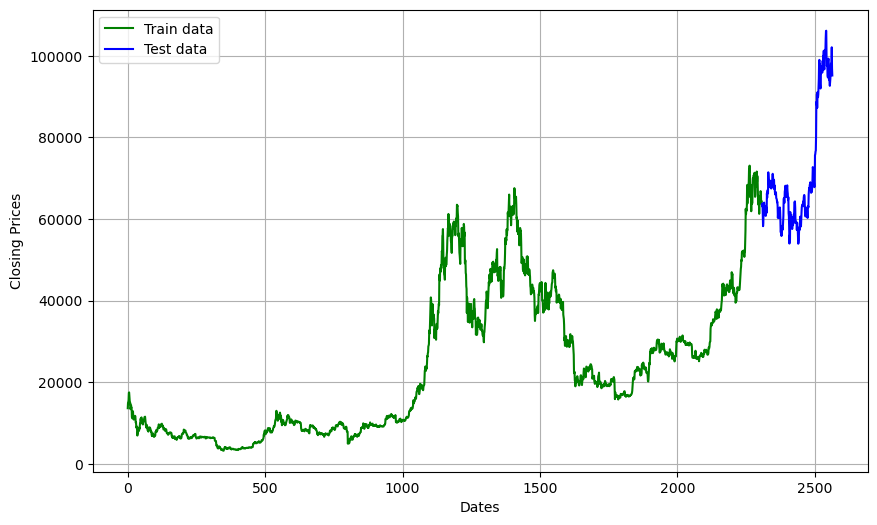
\includegraphics[keepaspectratio, width=0.95\textwidth]{pic/ar0.png}\\
        \end{center}
    \end{figure}
\end{frame}

\begin{frame}
    \frametitle{訓練したARIMAモデルとテストデータの対比}
    \begin{figure}[h]
        \begin{center}
            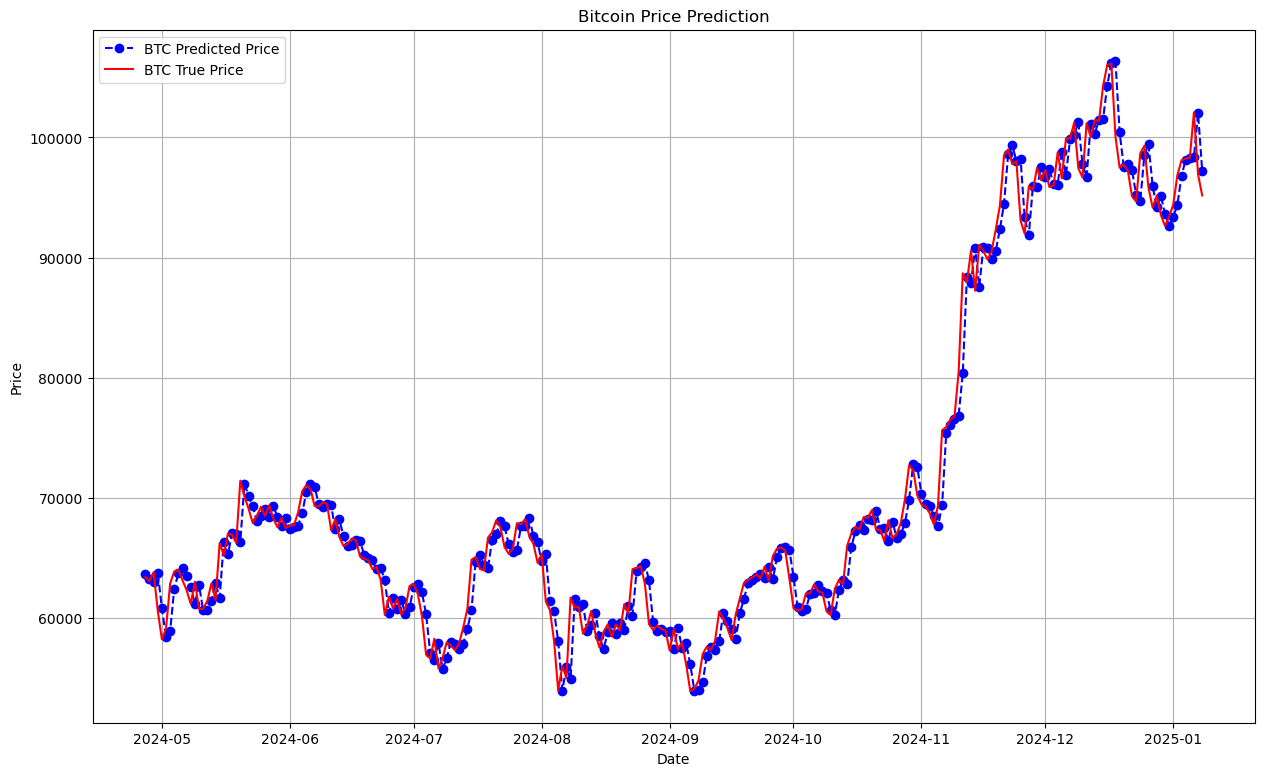
\includegraphics[keepaspectratio, width=0.95\textwidth]{pic/ar1.png}\\
        \end{center}
    \end{figure}
\end{frame}

\begin{frame}
    \frametitle{ARIMAモデルの評価}
    \begin{itemize}
        \item MAPE Value :1.94、すなわち、正確率は0.9806である
    \end{itemize}
\end{frame}


\begin{frame}
    \frametitle{ARIMAモデルでの未来1週間の価格予測}
    \begin{figure}[h]
        \begin{center}
            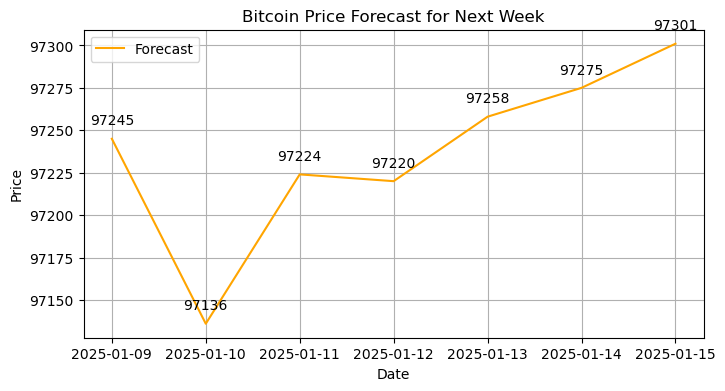
\includegraphics[keepaspectratio, width=0.95\textwidth]{pic/ar2.png}\\
        \end{center}
    \end{figure}
\end{frame}

\section{LSTM Model}

\subsection{ディープラーニング}
\begin{frame}
    \frametitle{データの標準化}
    \begin{figure}[h]
        \begin{center}
            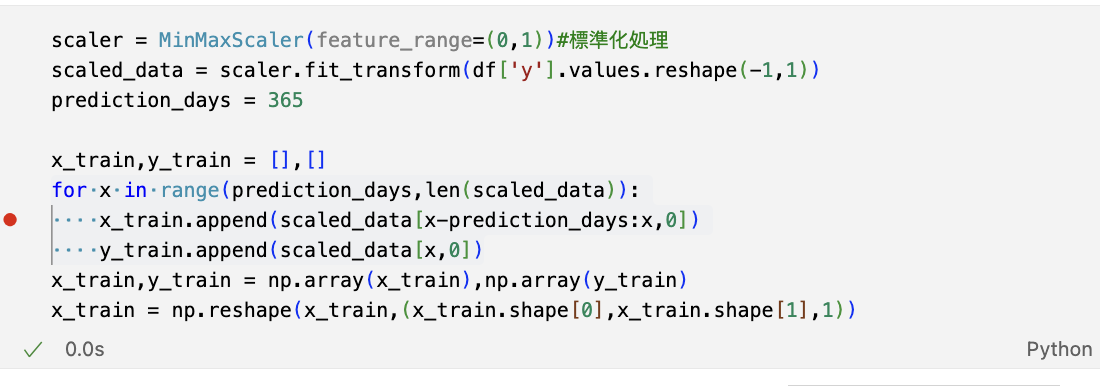
\includegraphics[keepaspectratio, width=0.95\textwidth]{pic/dl0.png}\\
        \end{center}
    \end{figure}
\end{frame}

\begin{frame}
    \frametitle{LSTMモデルの設定}
    \begin{figure}[h]
        \begin{center}
            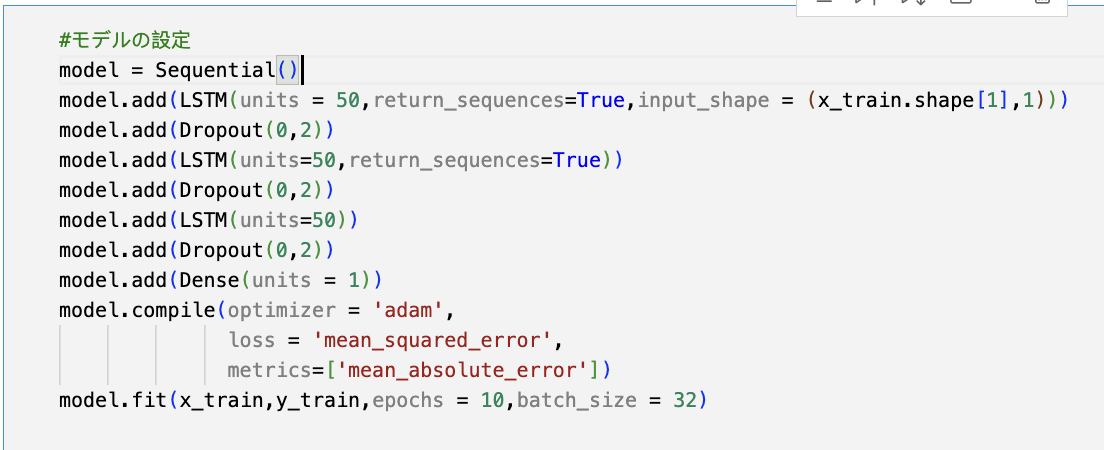
\includegraphics[keepaspectratio, width=0.95\textwidth]{pic/dl1.png}\\
        \end{center}
    \end{figure}
\end{frame}

\begin{frame}
    \frametitle{訓練したLSTMモデルとテストデータの対比}
    \begin{figure}[h]
        \begin{center}
            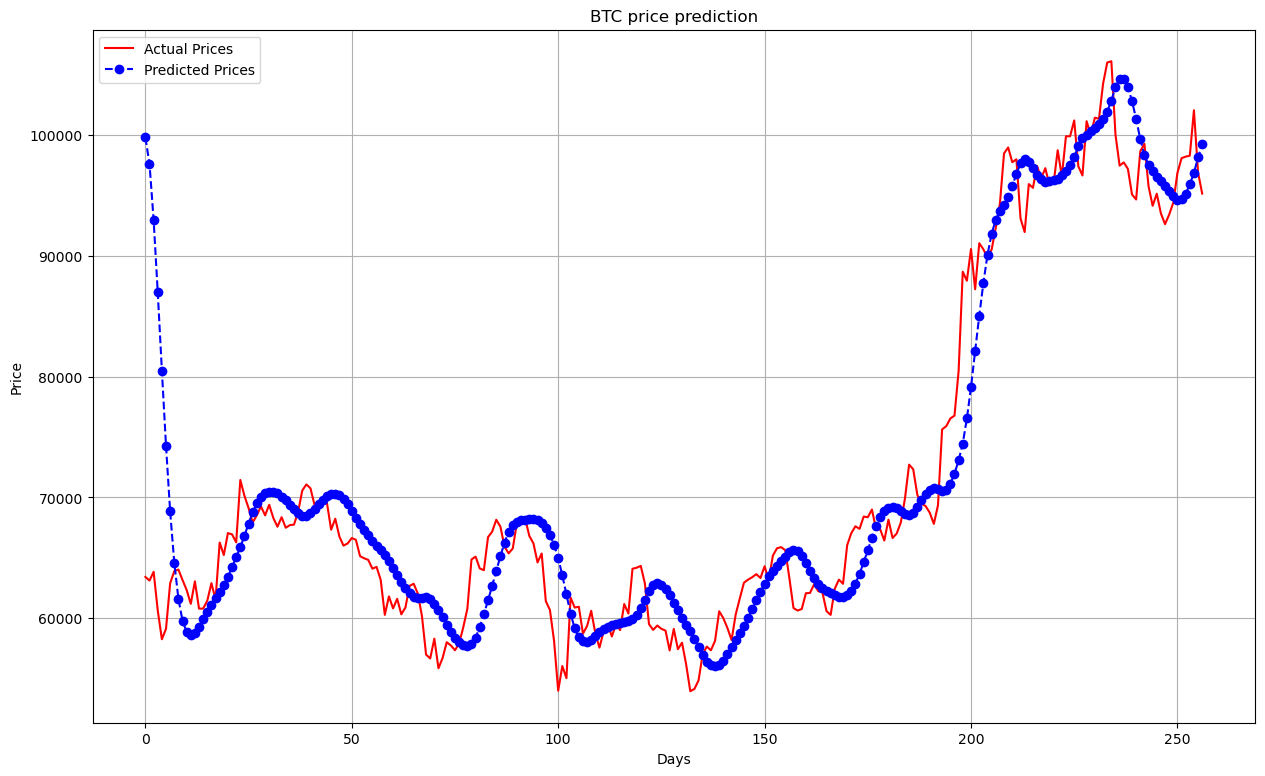
\includegraphics[keepaspectratio, width=0.95\textwidth]{pic/dl2.png}\\
        \end{center}
    \end{figure}
\end{frame}

\begin{frame}
    \frametitle{LSTMモデルの評価}
    \begin{itemize}
        \item MAPE Value :20、すなわち、正確率は0.8である
    \end{itemize}
\end{frame}

\section{References}
\begin{itemize}
    \item Prophetモデルの紹介は (https://www.skillupai.com/blog/tech/prophet) を参考してください
    \item Prophetの原理は(https://zhuanlan.zhihu.com/p/463183142)とコードの原理(https://zhuanlan.zhihu.com/p/52330017)を参考してください
    \item ARIMAモデルの原理の紹介は(https://datastudy.gonna.jp/arima/)を参考してください
    \item LSTMモデルの紹介は(https://qiita.com/KojiOhki/items/89cd7b69a8a6239d67ca)を参考してください
\end{itemize}

\begin{frame}
  \begin{center}
      {\Huge\calligra Thank You}
  \end{center}
\end{frame}

\end{document}
